\documentclass[../main.tex]{subfiles}
\begin{document}

\section{Board Setup}
Here we will walk through the different steps of setting up the board. Keep in mind that players can customize their maps in terms of size, elevation, and other factors to achieve the game play experience that best fits the preferences of their group.


\subsection{Step 1: Place the edges}
Place and interlock the Edges to create the play area of the board.

\begin{figure}[h]
    \centering
    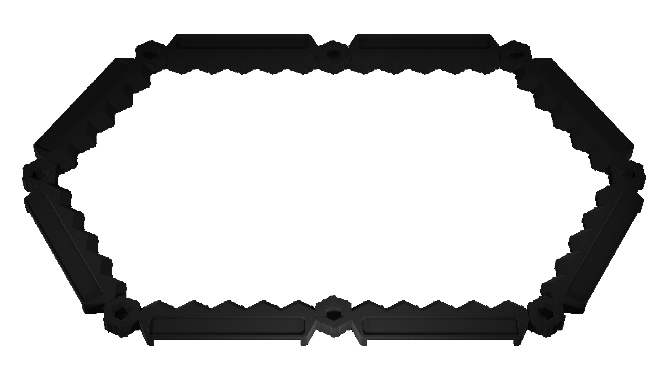
\includegraphics[width=1\linewidth]{chapters//boardsetup/Source Golf Edge Setup.png}
    \caption{Edge Setup}
\end{figure}

The Edges of the board are used to define the boundaries of the hole and to hold the dice. Feel free to play with the angles of the Edges to build many different shapes and sizes.



\textit{Recommendation: We recommend using eight Edges for a standard golf course experience.}

\subsection{Step 2: Build the Course}
For this section, you need to have the following hexes ready: 
\begin{itemize}
    \item 1 type of hex to act as the base.
    \item 1 type of hex to act as the water.
    \item 1 type of hex to act as the sand.
    \item 1 type of hex to act as the tee box and putting green. 
\end{itemize}


Place a base layer of hexes to play on. 

\begin{figure}[h]
    \centering
    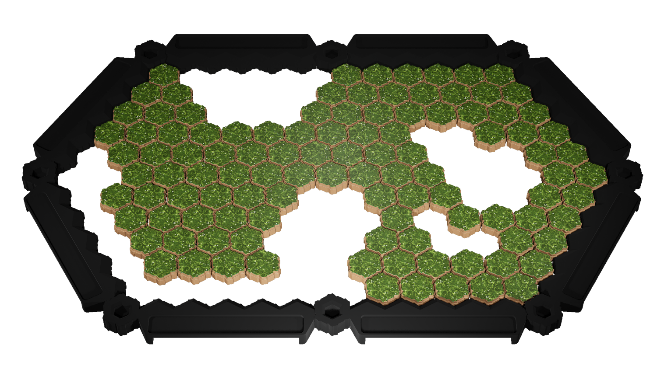
\includegraphics[width=1\linewidth]{chapters//boardsetup/Source Golf Base Layer.png}
\end{figure}

\textit{Recommendation: Use the larger multi-hexes to help build the base layer faster.}


Place water tiles to create lakes and rivers for the golf ball to fall into. 
\begin{figure}[h]
    \centering
    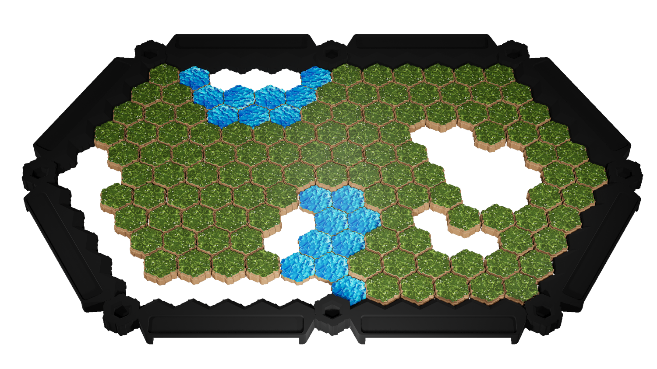
\includegraphics[width=1\linewidth]{chapters//boardsetup/Source Golf Base Layer Plus Water.png}
\end{figure}

Also place sand tiles that will act as bunkers.
\begin{figure}[h]
    \centering
    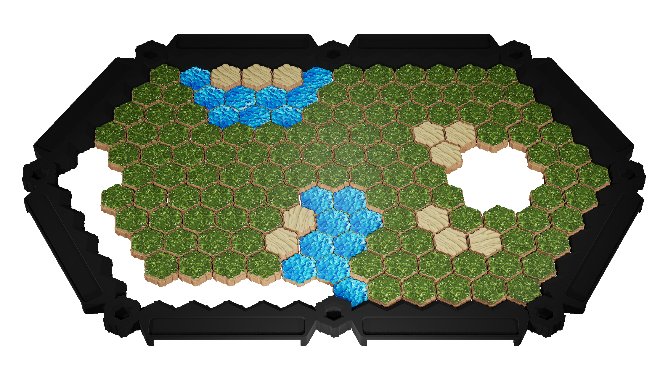
\includegraphics[width=1\linewidth]{chapters//boardsetup/Source Golf Base Layer.Water.SandTraps.png}
\end{figure}

Now set up the tee box and putting green. Choose one edge of the course to place the tee box. This can be 3 to 4 hexes together that allow multiple starting positions. Then pick a spot away from the tee box to place the putting green. This can be built with 7 or more hexes. 
\begin{figure}[h]
    \centering
    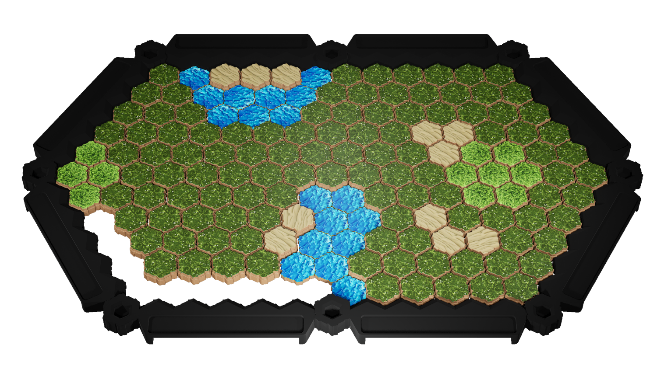
\includegraphics[width=1\linewidth]{chapters//boardsetup/Source Golf Base Layer.TeePuttingBox.png}
\end{figure}

Even add a little cart path. 
\begin{figure}[h]
    \centering
    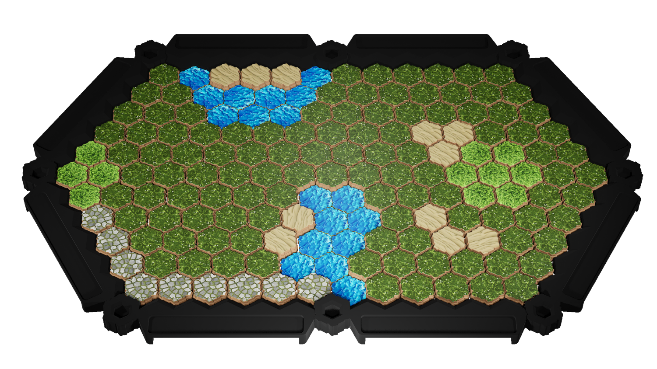
\includegraphics[width=1\linewidth]{chapters//boardsetup/Source Golf Base Layer.CartPath.png}
\end{figure}

\subsection{Step 3: Add Elevation and Obstacles}
Place additional land hexes to create height variances (elevation) on the course. 
 
\begin{figure}[h]
    \centering
    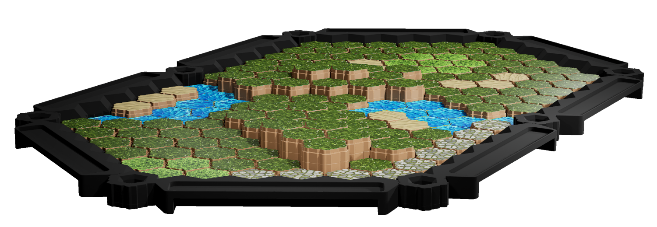
\includegraphics[width=1\linewidth]{chapters//boardsetup/Source Golf with Elevation.png}
\end{figure}
Elevation is a feature that can impact how the ball moves after it's been hit.

Other obstacles like trees can be added as well. 
\begin{figure}[h]
    \centering
    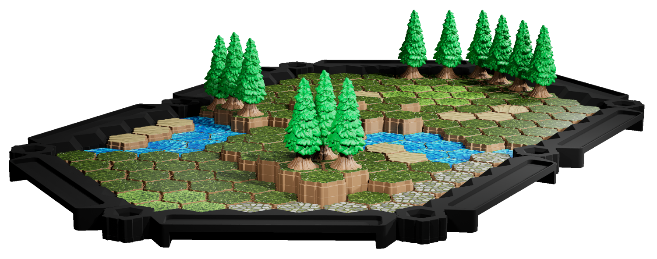
\includegraphics[width=1\linewidth]{chapters//boardsetup/Source Golf Base with Elevation.Trees.png}
\end{figure}

\subsection{Step 4: Place the Flag}
Place the flag miniature on one of the putting green hexes to represent the hole. 
\begin{figure}[h]
    \centering
    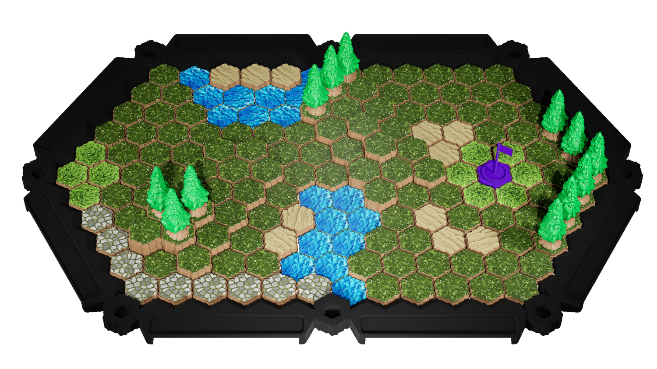
\includegraphics[width=1\linewidth]{chapters//boardsetup/Source Golf full hole topdown.png}
\end{figure}
\end{document}